\documentclass[twocolumn]{article}
\usepackage{graphicx} % Required for inserting images
\usepackage{booktabs}
\usepackage{pdflscape}
\usepackage{amsmath}
\usepackage{siunitx}
\usepackage{float}
\usepackage{url}
\usepackage{hyperref}
\usepackage[
    backend=biber,
    style=numeric
]{biblatex}
\addbibresource{Primo_BibTeX_Export.bib}
\hypersetup{
    colorlinks=true,
    linkcolor=blue,
    filecolor=magenta,      
    urlcolor=cyan,
    citecolor=blue,
    pdftitle={Overleaf Example},
    pdfpagemode=FullScreen,
    }
\usepackage{geometry}
\geometry{
 a4paper,
 total={170mm,257mm},
 left=20mm,
 top=20mm,
 }
\setcounter{secnumdepth}{0}
% \usepackage{float}
\title{STAT3006 A4}
\author{Avatar Azka - 47286238}
\date{November 2023}

\begin{document}

\onecolumn
\maketitle
{
    \hypersetup{linkcolor=black}
    \tableofcontents
    \newpage
    \listoffigures
    \listoftables
}

\newpage
\twocolumn
\section{Notes}

Aarøe et al. (2010) \cite{Aarøe2010} stated that the data had been standardised, however cursory examination of the data showed that the means and standard deviations of each feature did not match the expected values of standardised data (i.e. means were not equal to 0, standard deviations not equal to 1), which was odd. Thus, further Z-Score normalization was used to standardise the data. This was done in order to ensure all features are scaled similarly, such that features of different scales would not dominate (i.e. in PCA). 

\section{1. (5 Marks) PCA on Gene Expression Dataset}
Principal Component Analysis (PCA) was done on the dataset features to reduce the dimensions from 11217 genes to 121 principal components, which each represent a linear combination of the genes.

It is important to note that PCA does not take into account the output class when transforming the feature space. Indeed, in Figure \ref{fig:pp-pca}, we observe that the first 5 principal components by proportion of explained variance (which cumulatively explain $59\%$ of the data's variance) do not separate the classes as effectively as the methods described in later sections. The class distributions in each individual component, as well as pair-wise combinations of those components, exhibit much overlap between the normal and cancer classes. In the later sections, we will discuss other methods that better identify which genes are expressed differently between the normal and cancer groups.

The detailed results of each principal component's direction in terms of the original features can be found in \path{supplementary/PrincipalComponentDirections.csv}, which is a commas-separated values file where each row represents a principal component in descending order of proportion of explained variance. The first column of the file represents the index of the principal component, whereas every columns afterwards represents the coefficients of each original feature of the dataset in the linear combination that results in the principal component.

As for principal components that might be of interest to clinicians and scientists, that would require us to know which principal components best discriminate between normal and cancer classes, not just explain the greatest proportion of variance. To do this, Welch $t$-tests were conducted for each principal component to compare its significance with regards to the output class. The components were then sorted based on their p-values. These components and their direction with respect to the original genes are detailed in the file \path{supplementary/PrincipalComponentDirectionsByPval.csv}. The first 10 of these principal components are likely to be of interest to clinicians and scientists to further explore the correlation between the expressions of the genes most heavily weighed in said components and breast cancer.

To better visualize the separation between classes these principal components offer, Figure \ref{fig:pp-pca-significant} shows the class distributions for the top 5 principal components by order of significance according to their p-values. The class distributions in said figure show noticeably more separation compared to the top 5 principal components by order of proportion of explained variance, further reinforcing their significance to scientists and clinicians.

\begin{figure}[H]
    \centering
    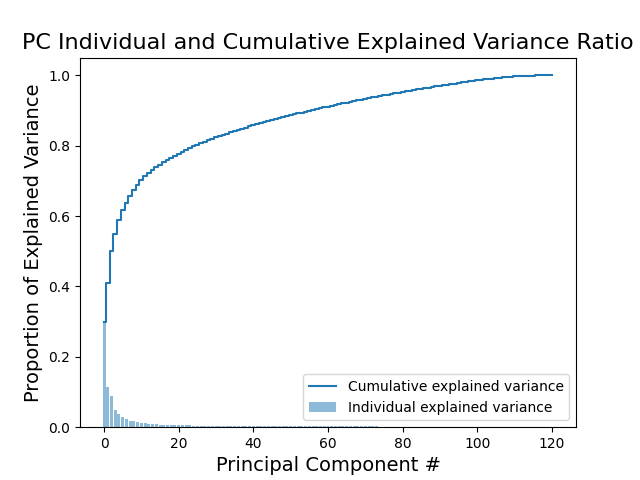
\includegraphics[width=\linewidth]{figures/PCA_Explained_Variance_Curve.png}
    \caption{Individual and cumulative proportions of variance explained by each component, sorted by descending order of explained variance ratio}
    \label{fig:pc-variance}
\end{figure}

\begin{figure}[H]
    \centering
    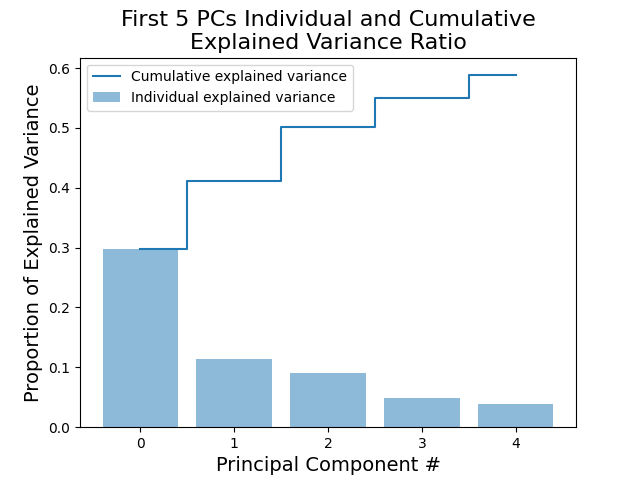
\includegraphics[width=\linewidth]{figures/PCA_Top_5_Explained_Variance_Curve.png}
    \caption{Individual and cumulative proportions of variance explained by the first 5 principal components, sorted by descending order of explained variance ratio}
    \label{fig:pc-variance-first-5}
\end{figure}


\section{2. (4 Marks) Single Variable Analysis}
Single Variable Analysis of this dataset was done by conducting Welch's $t$-tests on each feature for the two groups (i.e. normal and cancer) to calculate their $p$-values. Afterwards, the adjusted $p$-values were computed according to the Benjamini-Hochberg (1995) \cite{BenjaminiHochberg1995} procedure.

Exploratory use of the Benjamini-Yekutieli (2001) procedure was done in this dataset, though the process returned no genes below the threshold at all. It should be noted that Benjamini-Yekutieli is more conservative compared to Benjamini-Hochberg.

As the output is binomial, with continuous explanatory variables, Welch's $t$-test is suitable in this case. While Welch's $t$-test assumes normality of the feature distributions, it is fairly robust to non-normality in this data of this size \href{https://edstem.org/au/courses/13108/discussion/1697987}{(Ed \#259)}.

The Benjamini-Hochberg procedure assumes independence or positive dependency between test statistics. Benjamini \& Yekutieli (2001) \cite{BenjaminiYekutieli2001} state that in practice, dependent test statistics are encountered more often than independent ones. Here, it may be the case that certain genes exhibit collinearity. Indeed, Figure \ref{fig:pp-svm} shows an example of two closely related gene expressions, though it shows positive dependency, which does not violate Benjamini-Hochberg's assumptions.

It may be the case that this dataset, given its high dimensionality and possibility for gene expressions to be dependent on each other, does not fully meet the assumptions of Benjamini-Hochberg. If these assumptions are not met, then it is likely that the procedure will yield more false positives under the threshold.

The Benjamini-Hochberg procedure arranges the features based on ascending order of $p$-values, then computes a threshold, below which significant features are preserved. The threshold is defined as:

\begin{align*}
    P_{(j)} \leq FDR\cdot\frac{j}{m}
\end{align*}

Where $P_{(j)}$ represents the $p$-value of the $j$-th element in the ordered list of features, $FDR$ denotes the threshold for the False Discovery Rate we want to set, and $m$ is the total number of features we have. Figure \ref{fig:bh-threshold} visualises the Benjamini-Hochberg threshold versus the unadjusted $p$-values.

\begin{figure}[H]
    \centering
    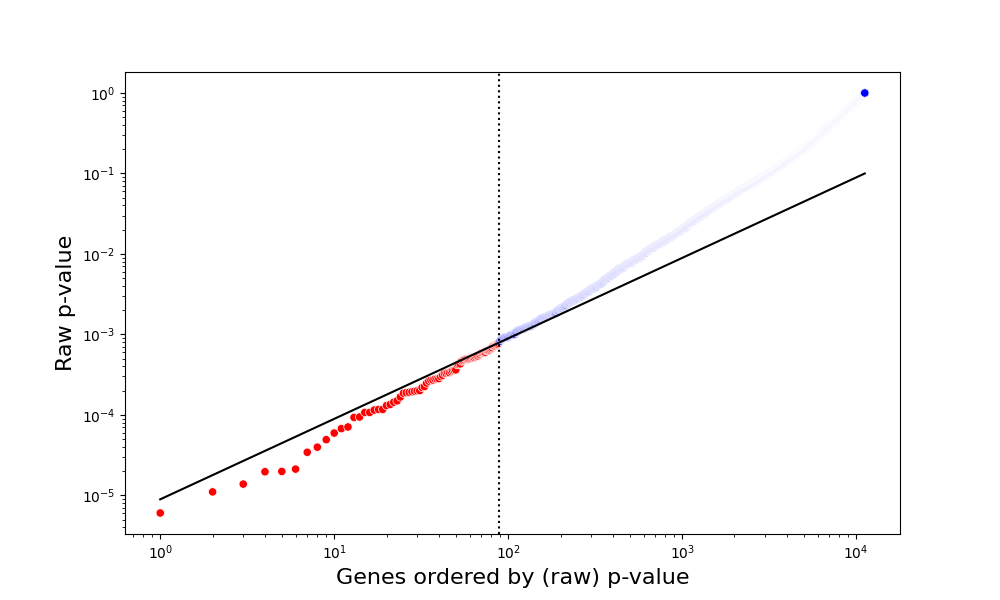
\includegraphics[width=\linewidth]{figures/SVA_Significant_Genes.png}
    \caption{Genes ordered by $p$-values $P_{(j)}$, and the line $0.1\cdot(j/11,217)$, representing the adjusted $p$-value threshold for the Benjamini-Hochberg method. Here the threshold lies at $j=88$, where the vertical dotted line is drawn.}
    \label{fig:bh-threshold}
\end{figure}

With the False Discovery Rate being capped to at most $0.1$, the Benjamini-Hochberg procedure yields $88$ significant genes, stopping at a maximum $p$-value of \num{7.76e-4}. A full list of the significant genes, along with their respective $p$-values can be found in \path{supplementary/SVASignificantGenes.csv}.

The genes deemed significant by the above SVA process represent genes whose differences in mean expression between classes differ at a statistically significant level. For this reason, the genes resulting from this procedure may be of interest to clinicians, scientists, and biologists for further research into how the difference in expression of these genes correlate to breast cancer.

\section{3. (3 Marks) Defining Binary Logistic Regression With Lasso Penalty}

Binary Logistic Regression in general seeks to maximise the log-likelihood:

\begin{align*}
    \ell(\beta) = \sum^{N}_{i=1}\left\{ y_i \beta^T x_i - \log\left(1 + e^{\beta^T x_i}\right) \right\}
\end{align*}

where $N$ is the number of observations, $y_i$ is the output class, $\beta$ are the coefficients for each feature, and $x_i$ is the vector of input variables.

Adding the $L_1$ (Lasso) penalty, the goal is then to find the coefficient vector $\beta$ and intercept $\beta_0$ maximise the penalised log-likelihood:

\begin{align*}
    \sum^{N}_{i=1}\left\{ y_i \beta^T x_i - \log\left(1 + e^{\beta^T x_i}\right) \right\} - \lambda \sum^{p}_{j=1}|\beta_j|
\end{align*}

where $p$ is the number of features, and $\lambda$ is the regularisation hyperparameter to tune the strength of regularisation (Hastie et al. 2009) \cite{HastieTrevor2009EoSL}. Higher values of $\lambda$ means stronger regularisation and thus, more shrinkage, essentially leading to more coefficients set to zero.

The traditional method to maximise the log-likelihood is the Newton-Raphson algorithm, though for more complex problems (large values of $N$ and $p$) GLMNET can instead be used, as mentioned in Hastie et al. (2009) \cite{HastieTrevor2009EoSL}. However, the method used in this report is an implementation of newGLMNET, developed by Yuan et al. (2012)\cite{JMLR:v13:yuan12a}, an optimization method based on GLMNET, provided by the LIBLINEAR library and implemented in \texttt{scikit-learn}.

\section{4. (3 Marks) Benefits \& Drawbacks of using PCA for Dimensionality Reduction}
PCA can reduce the dimensionality of the data by transforming its explanatory variables into principal components, whose values are linear combinations of the original explanatory variables that accounts for as much of the variance in the data as possible. 

In the context of being able to fit this transformed data to a classifier, this comes with several benefits. Some models (for example, LDA or linear regression if unregularised) are entirely unable to fit the original data if $p>n$. PCA brings down the number of features such that $p \le n$. This comes with the added benefit of potentially reducing the effect of overfitting, especially if one reduces the amount of principal components to cover at least a certain percentage of the data's variance. Models trained on and evaluating this transformed feature space will also tend to run faster, such is the case with a K-Nearest Neighbors classifier, for example, where its time complexity is $O(np)$. Furthermore, representing the original features as principal components allows for visualisation of the data in lower dimensions whilst still accounting for the features that compose the principal components.

However, reduction of the data's feature space comes with the downside of reduced interpretability. Since each principal component represents a linear combination of multiple features, it makes it harder to identify which individual features show significant difference in value between classes. Furthermore, PCA reduces the dimensionality of the data solely based on maximising explained variance, and does not take into account the output class. Therefore, principal components that explain a large proportion of the data's variance may not necessarily reflect how powerful those components are in discriminating between classes.

For the problem being explored in this report, I have chosen not to use PCA for the classifiers in the following section. This is because the models chosen (i.e. Lasso-penalised Logistic Regression and Linear-Kernel Support Vector Machine) handle high dimensional data well (Hastie et al. 2009) \cite{HastieTrevor2009EoSL}, and reducing the feature space into principal components in this case will simply make it harder to identify the significant genes that scientists may use as discriminating indicators for cancer diagnosis.

\section{5. Classification}

The models used in this section are the Lasso-penalised Logistic Regression (henceforth LLR) and Support Vector Machine (SVM) Classifiers. 

For the LLR classifier, the regularisation hyperparameter $\lambda$ for the LLR classifier was determined via nested cross validation, as explained in section 5c.

The SVM classifier utilized a linear kernel, as informed by Hastie et al. (2009) (p.659) \cite{HastieTrevor2009EoSL}, where the authors state that while the aim of fitting nonlinear decision boundaries for SVM classifiers, such models are already sufficiently complex in cases where $p \gg N$. The regularisation hyperparameter $C$ for the SVM classifier is left as the default value $1.0$. This was based on Hastie et al. (2009) (p.658) \cite{HastieTrevor2009EoSL} in which the authors state that error rates for SVM classifiers on high dimensional data are insensitive to the choice of the regularisation hyperparameter. 

\subsection{a. (1 Marks) Characterisation of Each Class}

We can make characterisations of each class by examining both the confusion matrices of each classifier, as well as the computed coefficients of each feature. 

Figures \ref{fig:cm-lasso} and \ref{fig:cm-svm} show the confusion matrices for the LLR and SVM classifiers respectively. Notably, the LLR classifier errs more towards false positives (predicting cancer where it should be normal) than the SVM classifier does. Conversely, the SVM classifier errs more towards false negatives. 

The files \path{supplementary/GeneImportanceLasso} and \path{supplementary/GeneImportanceSVM} detail which genes each classifier deems most significant in terms of its ability to discriminate between the normal and cancer classes.

\begin{figure}[H]
    \centering
    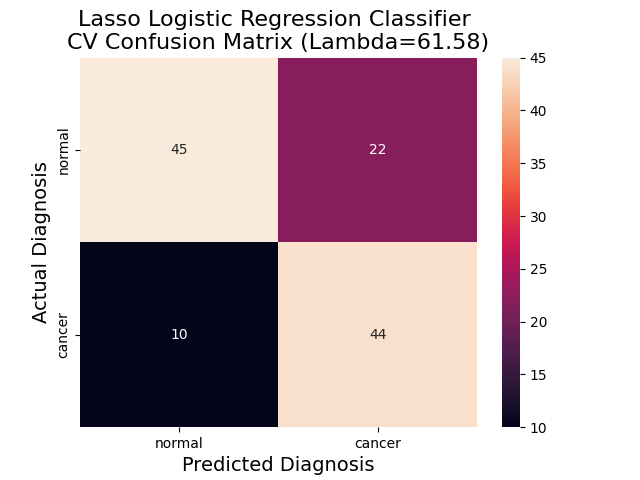
\includegraphics[width=\linewidth]{figures/Lasso_Logistic_Regression_Classifier_CV_Confusion_Matrix.png}
    \caption{Confusion matrix for the LLR classifier, estimated via 10-fold CV with $\lambda = 61.58$ (see section 5c for how this value was determined)}
    \label{fig:cm-lasso}
\end{figure}

\begin{figure}[H]
    \centering
    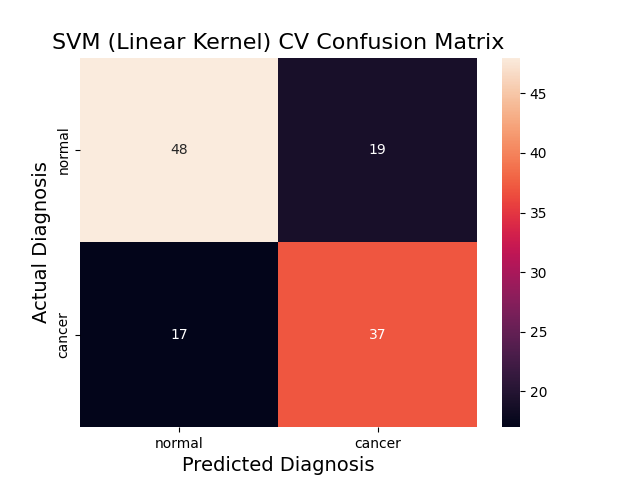
\includegraphics[width=\linewidth]{figures/SVM_(Linear_Kernel)_CV_Confusion_Matrix.png}
    \caption{Confusion matrix for the SVM classifier, estimated via 10-fold CV}
    \label{fig:cm-svm}
\end{figure}

\subsection{b. (2 Marks) CV-based Error Rate Estimates}
10-fold Cross Validation was used to compute the overall and class-specific error rates of each classifier. The results are as follows:

\begin{table}[H]
    \centering
    \begin{tabular}{lrrrr}
    \toprule
     & precision & recall & f1-score & support \\
    \midrule
    cancer & 0.82 & 0.67 & 0.74 & 67 \\
    normal & 0.67 & 0.81 & 0.73 & 54 \\
    accuracy & & & 0.73 & 121 \\
    \bottomrule
    \end{tabular}
    \caption{LRR 10-fold CV error rates}
    \label{tab:errors-lrr}
\end{table}

\begin{table}[H]
    \centering
    \begin{tabular}{lrrrr}
    \toprule
     & precision & recall & f1-score & support \\
    \midrule
    cancer & 0.74 & 0.72 & 0.73 & 67\\
    normal & 0.66 & 0.68 & 0.67 & 54\\
    accuracy & & & 0.70 & 121 \\
    \bottomrule
    \end{tabular}
    \caption{SVM 10-fold CV error rates}
    \label{tab:errors-svm}
\end{table}

Both classifiers, when trained on all the data, perfectly predict the class of each sample in the dataset, thus the error rates in this case are trivial and are not included.

\subsection{c. (3 Marks) Finding The Optimal Value of Lambda}
Nested Cross Validation was done over a predetermined search space of potential values of $\lambda$ for the LRR classifier. The search space consists of 20 potential values for lambda, spread evenly on a log scale between $\num{1e-3}$ to $\num{1e4}$. A full list of the search space can be found in the appendix as Table \ref{tab:lambda-search-space}. 

The accuracy of the LLR classifier over all folds for all values of $\lambda$ in the search space were recorded, and the value of $\lambda$ which yielded the best accuracy score was then used for the final LLR classifier. The error rates reported in Table \ref{tab:errors-lrr} represent the inner-loop 10-fold CV where the optimal $\lambda$ was used. In this case, $\lambda=61.58$ showed the greatest reported CV accuracy estimate, as reported in Table \ref{tab:errors-lrr}.

\begin{figure}[H]
    \centering
    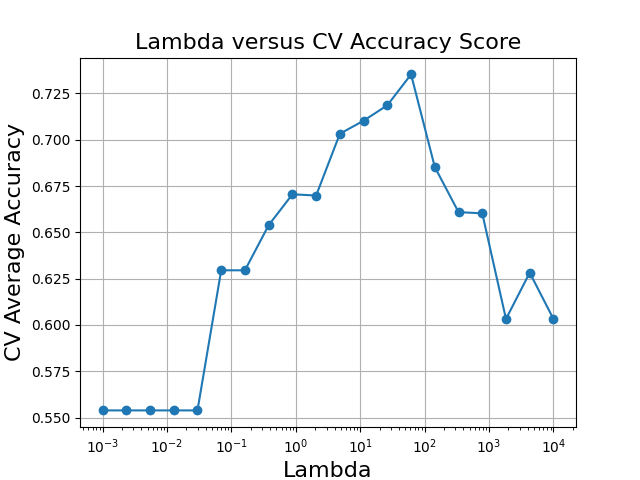
\includegraphics[width=\linewidth]{figures/Lambda_versus_CV_Accuracy_Score.png}
    \caption{Impact of the choice of the LLR regularisation hyperparameter $\lambda$ on the accuracy of the classifier. Here, the x axis is set to a log scale to reflect the logarithmic search space over potential values of $\lambda$}
    \label{fig:lambda-search}
\end{figure}

A list of the top 30 (truncated for space) genes ordered by importance according to their corresponding coefficients in the final LLR classifier is listed in the appendix as Table \ref{tab:genes-lasso}. A more complete list of all the sorted genes and their coefficients is available in \path{supplementary/GeneImportanceLasso} as a commas-separated values file. In all, the LLR classifier identified 394 important genes, in that those genes had nonzero coefficients in the classifier.

A list of the top 30 genes (truncated for space) for the SVM classifier, trained on the entire dataset, can be found in the appendix as Table \ref{tab:genes-svm}. A more complete list, such as that of LLR's, can be found in \path{supplementary/GeneImportanceSVM}

Each classifier showed overall apparent error rates, when trained on all the data and applied back to it, of $100\%$ accuracy. This could mean a high degree of bias in both classifiers, implying the classifier overfits the training data.

\section{6. (4 Marks) Results Comparison}

Figures \ref{fig:pp-pca}, \ref{fig:pp-pca-significant}, \ref{fig:pp-lasso}, \ref{fig:pp-svm}, \ref{fig:pp-sva} in the Appendix (also available in \path{figures/PairPlot*} in the supplementary files) show plots of class distributions over pairs of features and principal components deemed significant by each analytical method. From these pair plots we can see a visual representation of how well these methods identify genes that are expressed differently between the cancer and normal groups, both individually (in each of the plots' main diagonals) and pair-wise.

Visually, it can be observed that most of the methods explored in this report are able to identify genes that are expressed differently between normal and cancer patients, which is the main goal of this exploration, and allows further research into the link between these genes and breast cancer, as well as diagnosis via blood sample alone. 

This is with the notable exception of the top 10 principal components, in order of explained variance ratio. Since PCA is not informed of the output classes, it does not provide very helpful insights into genes that can discriminate between classes.

To quantify the discriminative power of the genes produced by each of the methods used, a Logistic Regression classifier with L2 regularisation was fit to the top 10 genes from each method. Via 10-fold CV we observe the Area Under the Receiver Operating Characteristic Curve (AUC) score for each set of genes, detailed in Table \ref{tab:auc-scores}. Aaroe et al. (2010) \cite{Aarøe2010} used a similar approach in using AUC scores to measure separation between groups.

\begin{table}[H]
    \centering
    \begin{tabular}{ll}
    \toprule
    Top 10 Genes/PC Origin & AUC Score\\
    \midrule
    LRR & 0.86\\
    SVM & 0.86\\
    SVA & 0.80\\
    PCA & 0.58\\
    PCA (by $p$-value) & 0.80\\
    \bottomrule
    \end{tabular}
    \caption{10-Fold CV AUC scores for the logistic regression model, trained only on the top 10 genes/principal components from each method. A high AUC score $(>0.8)$ denotes good separation between classes, whereas $(0.5)$ indicates the model to be on par with being correct by chance (e.g. a coin toss).}
    \label{tab:auc-scores}
\end{table}

Again, we see PCA lacking in its ability to identify genes whose expressions are different in each class. Though, to be fair, it isn't its explicit purpose. Regardless, its use here makes it difficult to identify which individual genes are correlated with breast cancer.

The top 10 genes chosen by SVA show good discriminative power individually, owing to its difference in means between classes, as identified by their $p$-values. However, this doesn't tell us the whole story. SVA may excel at identifying individual genes that express differently in cancer and non-cancer patients, but may not necessarily give us combinations of features that may better separate the classes than they do on their own. Analysis via classifier coefficients such as using LLR and SVM allow us to identify features that, when weighed together as part of a combination, best predict the class.

Any 10 genes from the top 10 genes produced by LRR, SVM, and SVA (All shown in Table \ref{tab:top-all}) show promise, should a scientist wish to study the link between their expressions and breast cancer, as they all show discriminative power between classes. In particular, if one wishes to further study genes that are expressed differently between the two groups individually, they may want to take a look at the top 10 genes produced by SVA. On the other hand, should they want to identify genes that express differently as part of a combination between the two groups (perhaps to build a model to predict the class of new observations, or to examine how interactions between those gene expressions correlate with breast cancer), then the top 10 genes in each of the classifiers show great promise.

\begin{table}[H]
    \centering
    \begin{tabular}{llll}
    \toprule
    Rank & lasso & svm & sva \\
    \midrule
    1 & 105982 & 105982 & 134910 \\
    2 & 162796 & 186433 & 168498 \\
    3 & 710141 & 107457 & 107457 \\
    4 & 229944 & 216357 & 207178 \\
    5 & 182204 & 168498 & 192905 \\
    6 & 221030 & 213145 & 208343 \\
    7 & 106478 & 192006 & 200120 \\
    8 & 192905 & 156497 & 177738 \\
    9 & 168498 & 712587 & 110790 \\
    10 & 186433 & 125981 & 149826 \\
    \bottomrule
    \end{tabular}
    \caption{Top 10 Genes from LRR, SVM, and SVA, in descending order of significance}
    \label{tab:top-all}
\end{table}

\newpage
\printbibliography[
    heading=bibintoc,
    title={References}
]

\newpage
\onecolumn
\section{Appendix}
\subsection{5c. Lambda Search Space}
\begin{table}[H]
    \centering
    \begin{tabular}{cccc}
        1.00e-03& 2.33e-03& 5.45e-03& 1.27e-02 \\
        2.97e-02& 6.95e-02& 1.62e-01& 3.79e-01 \\
        8.85e-01& 2.06e+00& 4.83e+00& 1.12e+01 \\
        2.63e+01& 6.15e+01& 1.43e+02& 3.35e+02 \\
        7.84e+02& 1.83e+03& 4.28e+03& 1.00e+04 \\
    \end{tabular}
    \caption{20 potential values for $\lambda$, spread evenly on a log scale between $\num{1e-3}$ to $\num{1e4}$}
    \label{tab:lambda-search-space}
\end{table}

\subsection{5c. Gene Importance}
\begin{table}[H]
    \centering
    \begin{tabular}{lr}
    \toprule
    Gene & coef \\
    \midrule
    105982 & 0.567246 \\
    162796 & 0.488020 \\
    710141 & 0.470698 \\
    229944 & -0.457330 \\
    182204 & 0.449716 \\
    221030 & -0.439259 \\
    106478 & -0.439046 \\
    192905 & 0.431565 \\
    168498 & 0.412588 \\
    186433 & 0.394274 \\
    156497 & -0.390394 \\
    185593 & 0.383622 \\
    180577 & 0.380414 \\
    187446 & -0.373134 \\
    125981 & 0.372778 \\
    213145 & -0.361821 \\
    222840 & 0.357356 \\
    208243 & 0.355445 \\
    127723 & 0.353830 \\
    150701 & -0.349412 \\
    107457 & -0.339129 \\
    151002 & -0.333791 \\
    115418 & -0.331658 \\
    216357 & -0.304303 \\
    243149 & -0.302698 \\
    196441 & -0.299391 \\
    180804 & 0.292722 \\
    203708 & 0.289368 \\
    203664 & 0.288367 \\
    104116 & 0.282697 \\
    \bottomrule
    \end{tabular}
    \caption{Top 30 genes sorted by importance based on the absolute value of its coefficient in the LLR classifier. A full list of these genes and their respective coefficients can be found in \path{supplementary/GeneImportanceLasso}}
    \label{tab:genes-lasso}
\end{table}

\begin{table}[H]
    \centering
    \begin{tabular}{lr}
\toprule
Gene & coef \\
\midrule
105982 & 0.010418 \\
186433 & 0.008755 \\
107457 & -0.008699 \\
216357 & -0.008481 \\
168498 & 0.007978 \\
213145 & -0.007974 \\
192006 & -0.007699 \\
156497 & -0.007496 \\
712587 & -0.007415 \\
125981 & 0.007395 \\
229944 & -0.007359 \\
192905 & 0.007352 \\
115418 & -0.007350 \\
137563 & 0.007341 \\
134910 & -0.007161 \\
157702 & 0.007119 \\
203664 & 0.007104 \\
107385 & 0.007001 \\
147346 & -0.006961 \\
180577 & 0.006936 \\
710141 & 0.006798 \\
221030 & -0.006747 \\
185593 & 0.006744 \\
106478 & -0.006660 \\
228421 & -0.006562 \\
235219 & -0.006530 \\
196441 & -0.006481 \\
149070 & 0.006441 \\
203708 & 0.006424 \\
243149 & -0.006406 \\
\bottomrule
\end{tabular}
    \caption{Top 30 genes sorted by importance based on the absolute value of its coefficient in the SVM classifier. A full list of these genes and their respective coefficients can be found in \path{supplementary/GeneImportanceSVM}}
    \label{tab:genes-svm}
\end{table}


\subsection{6. Class Distribution Pair Plots}
\begin{figure}[H]
    \centering
    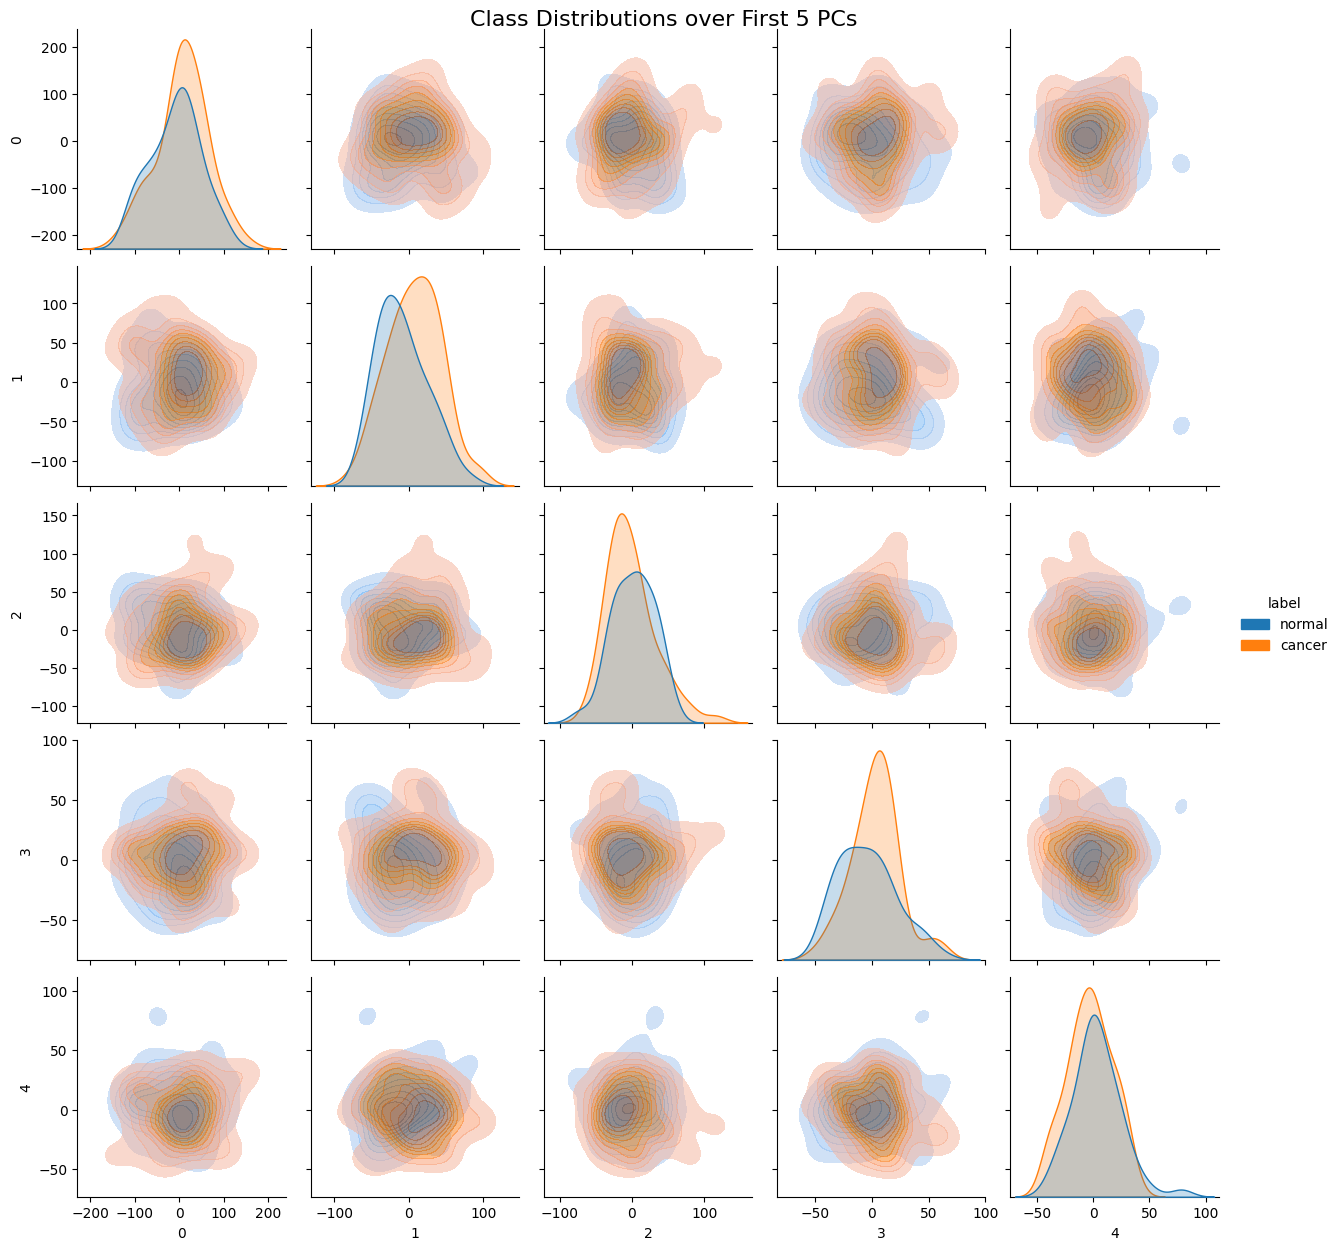
\includegraphics[width=0.85\linewidth]{figures/PairPlot_PCA.png}
    \caption{Pair plot of class distributions over the first 5 principal components in order of explained variance ratio}
    \label{fig:pp-pca}
\end{figure}

\begin{figure}[H]
    \centering
    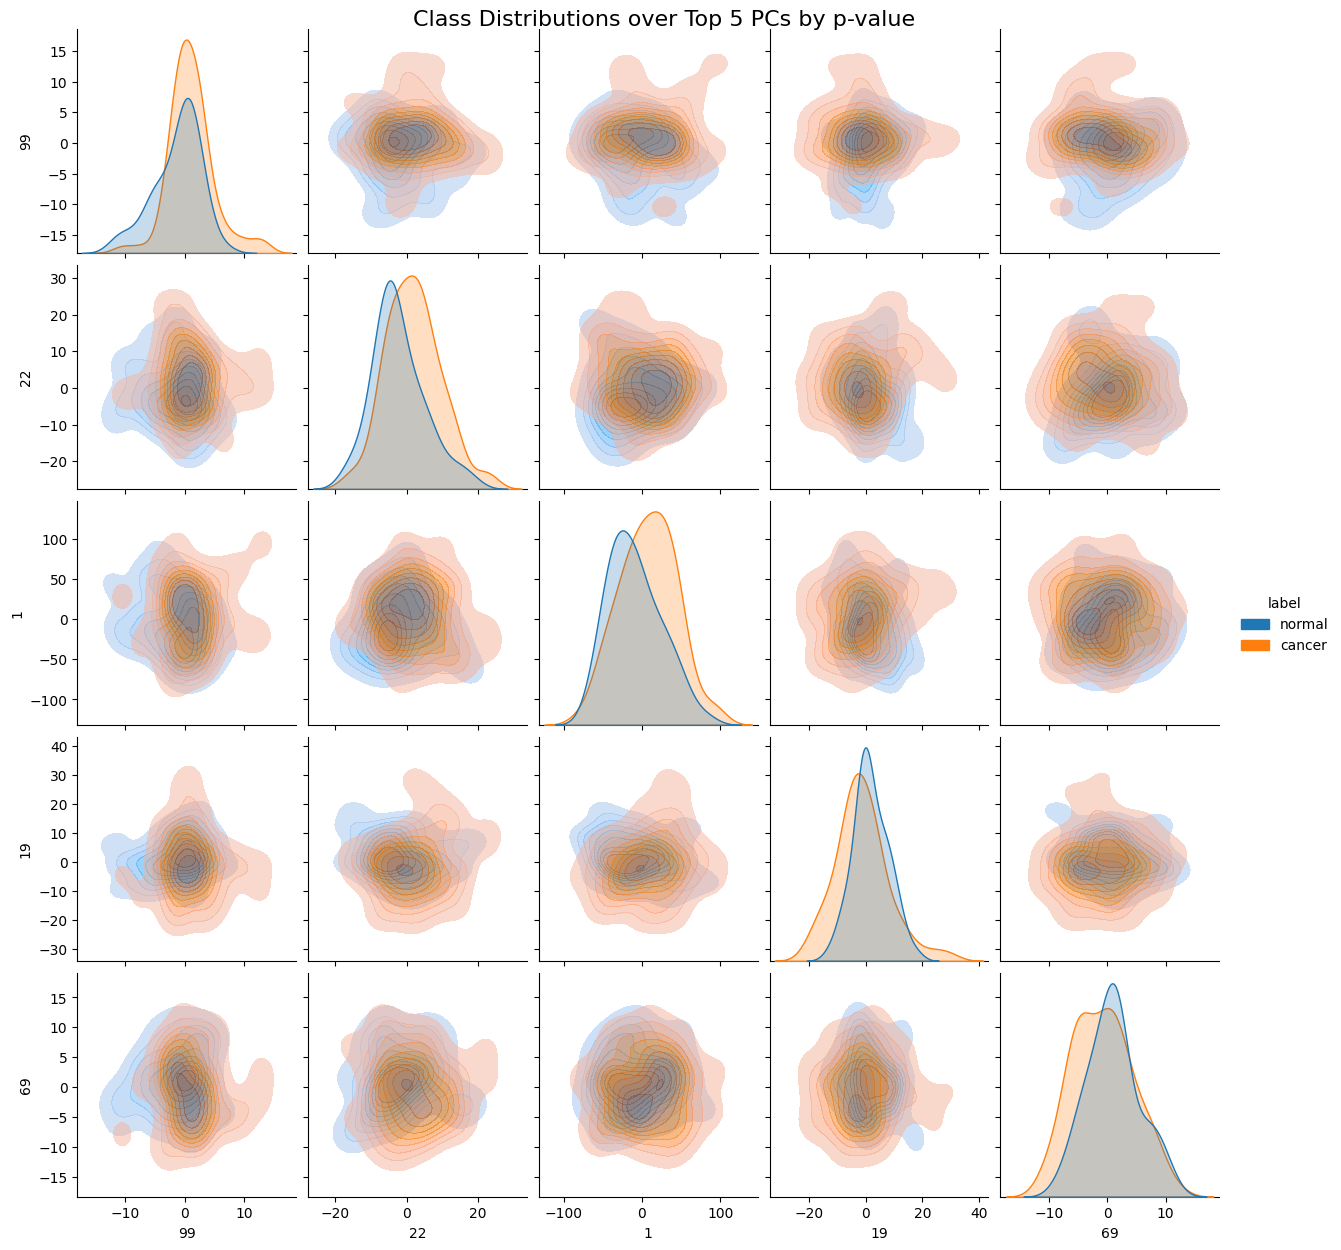
\includegraphics[width=0.85\linewidth]{figures/PairPlot_PCA_Significant.png}
    \caption{Pair plot of class distributions over the top 5 principal components in order of p-value}
    \label{fig:pp-pca-significant}
\end{figure}

\begin{figure}[H]
    \centering
    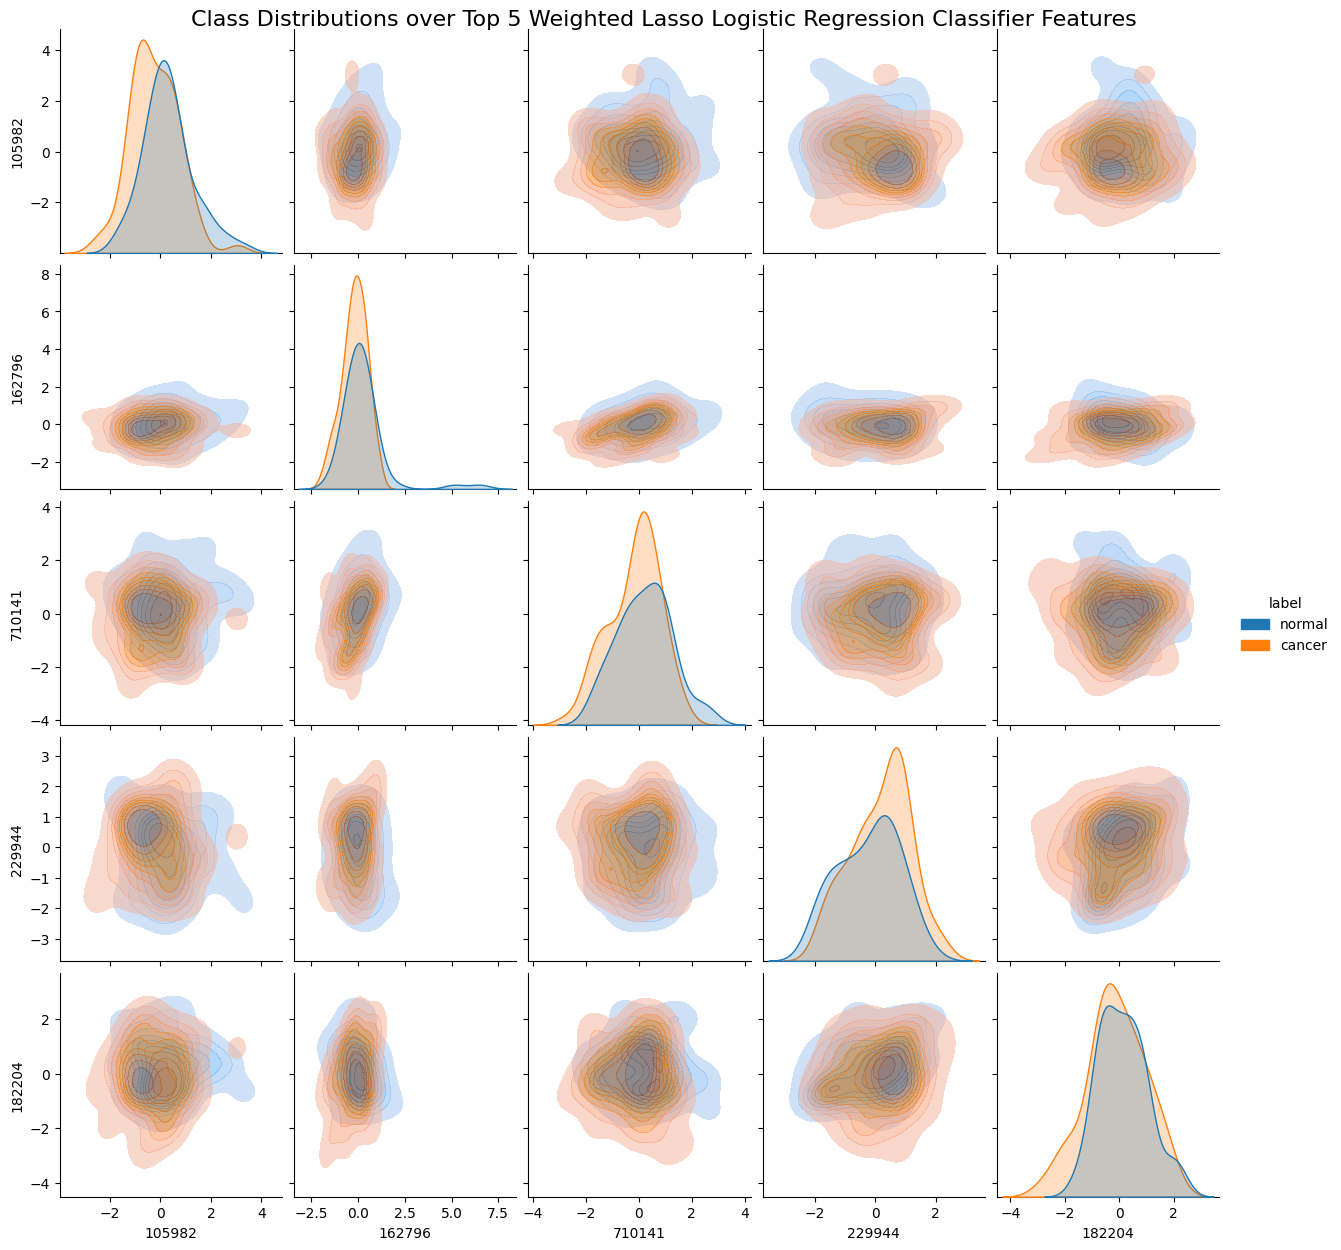
\includegraphics[width=0.85\linewidth]{figures/PairPlot_Lasso.png}
    \caption{Pair plot of class distributions over the top 5 weighted features in the LLR classifier}
    \label{fig:pp-lasso}
\end{figure}

\begin{figure}[H]
    \centering
    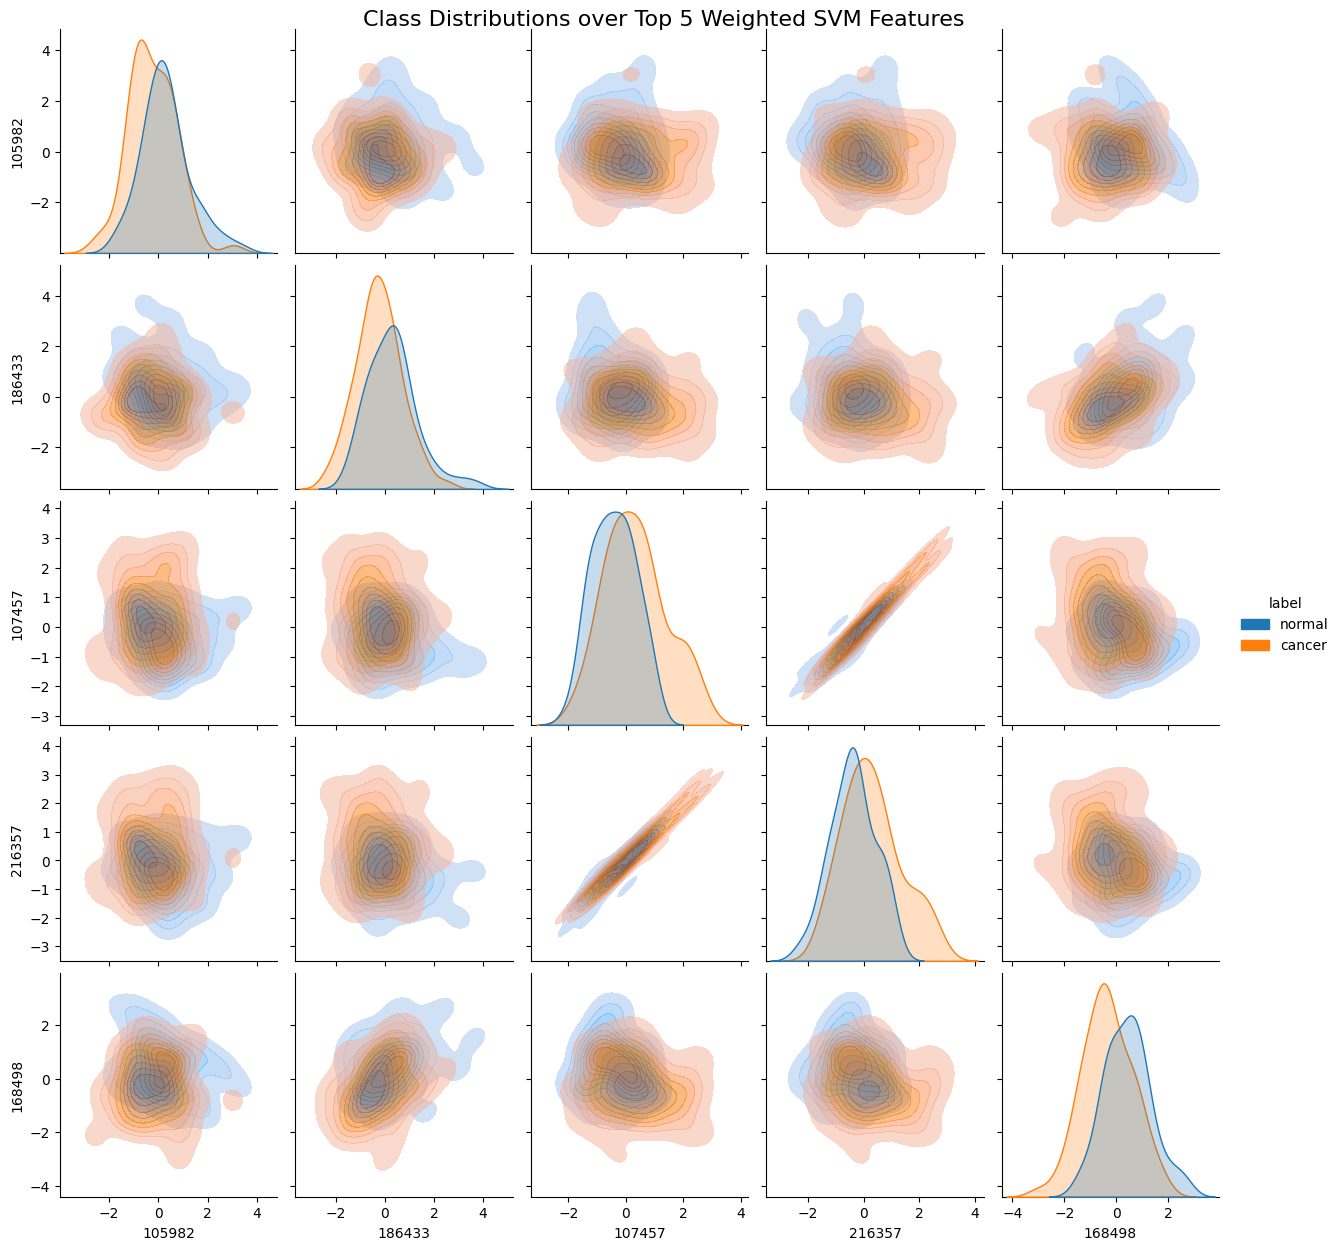
\includegraphics[width=0.85\linewidth]{figures/PairPlot_SVM.png}
    \caption{Pair plot of class distributions over the top 5 weighted features in the SVM classifier}
    \label{fig:pp-svm}
\end{figure}

\begin{figure}[H]
    \centering
    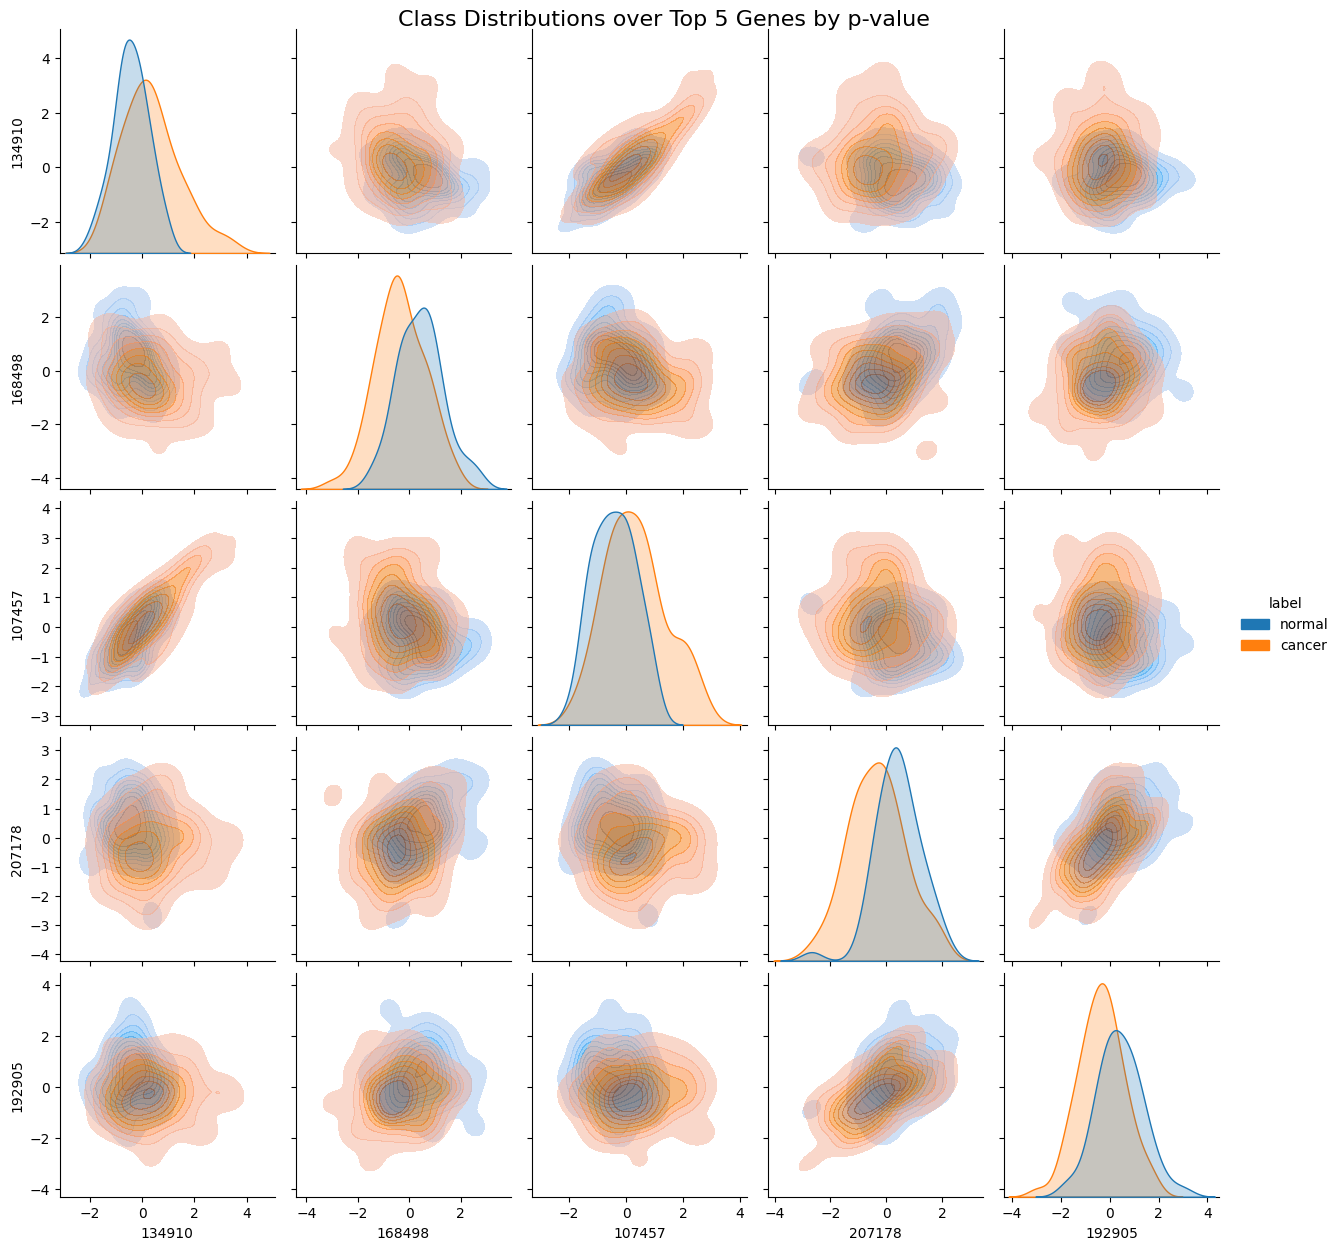
\includegraphics[width=0.85\linewidth]{figures/PairPlot_SVA.png}
    \caption{Pair plot of class distributions over the top 5 significant features based on p-value}
    \label{fig:pp-sva}
\end{figure}

\end{document}